% article example for classicthesis.sty
\documentclass[10pt,a4paper]{article} % KOMA-Script article scrartcl
\usepackage{lipsum}
\usepackage{url}
\usepackage[nochapters]{../classicthesis} % nochapters
\usepackage{graphicx}
%\graphicspath{ {images/} }
\usepackage{booktabs}
\usepackage{float}








\usepackage{hyperref}

\begin{document}
    \pagestyle{plain}
    \title{\rmfamily\normalfont\spacedallcaps{Mission: Chuckhole}}
    \author{\spacedlowsmallcaps{Marwan ElMezni, Michael Moosbauer}}
    \date{} % no date
    
    \maketitle
    
%    \begin{abstract}
        %Maybe we won't need an abstract
 %   \end{abstract}
       
    \tableofcontents
\newpage    
    \section{Motivation and problem statement}



Even though municipalities try to maintain and repair roads, many segments still contain chuckholes that vehicle owners prefer to avoid to drive or to bike on because they would so likely damage their vehicles and slow or interrupt the traffic.

This was the background motivation to develop a mobile application, in a biking context, that helps users to avoid damaged sections of roads or to detect and localize chuckholes.

 
 
 
 
    \section{Recommended Setup}
	%photo of bike, smartphone fix, ...    
	\begin{itemize} 
	\item Bike: Drössiger 650B full suspension.
	\item Smartphone (Samsung Galaxy S4 Active).
	\item Fix spot of the mobile phone: on the handlebar.
	
	
	\end{itemize}
	% send me a picture of your bike with the fix and the phone


    \section{Architecture and flow of information}
	% maybe UML class diagram, if suitable
	
	\begin{figure}[H]
	\centering
    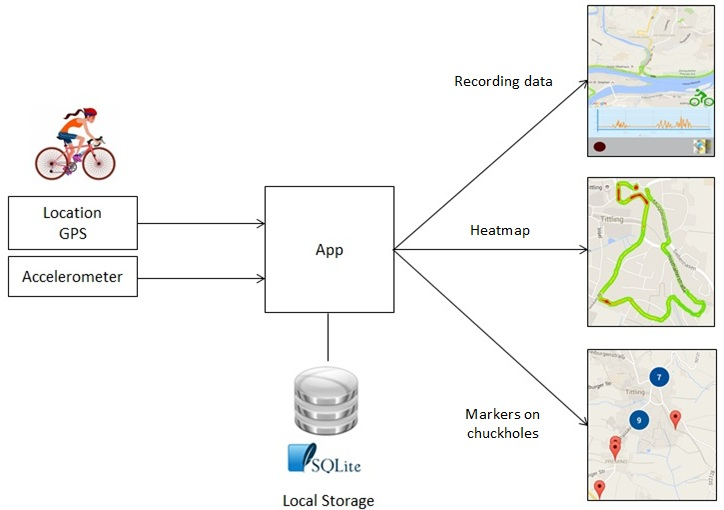
\includegraphics[width=16cm, height=12cm]{pic1}
    
    \end{figure}
    
    
    
    
    \section{App Features}
	% pictures etc. here
    
    \subsection{ Recording data}
    
    
    
    
    \subsection{ Heatmap Overlay}
    
    Heatmaps make it easy for viewers to understand the distribution and relative intensity of data points on a google map and was overlaid using the Google Maps Android Heatmap Utility.
    We opted for a dynamic heatmapping that requires a collection of 'weighted' latitude/longitude coordinates, each with an intensity value that will determine its associated color.
    Highest values of intensity will be mapped by default to red while lowest ones to green. Concerning the values in between, the given color is generated using interpolation between red and green. 
    Our collection will retrieve locations from the DataStore structure and their corresponding g-force values which will represent the intensity parameter. Consequently, locations on a smooth road will get green color while chuckholes will be colored in red and points with average g-forces values will be in yellow.
     
    \begin{figure}[H]
    \centering
	
	  
	   
       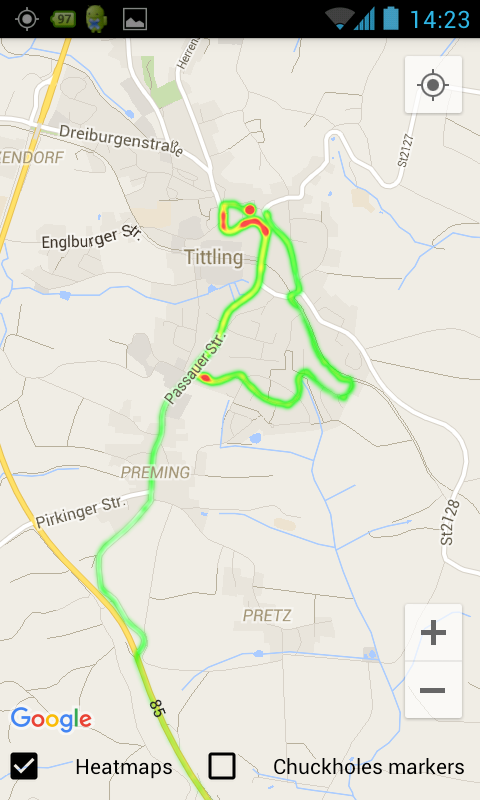
\includegraphics[width=5cm, height=8cm]{pic4}
    
       
        \end{figure}
    
    Unfortunately, the heatmap utility suffers from some limitations that are described in the following article: 
    \url{http://cartographicperspectives.org/index.php/journal/article/view/cp80-deboer/1420}. The main handicap that affects our overlay is that the heatmaps circles overlap at low zoom levels which causes fake coloring and this is due to the fact that the 'Intensity' parameter is additive: the overlap area of two circles of intensity 1 will lead to an overall intensity 2.
    \begin{figure}[H]
    \centering
	
	  
	   
       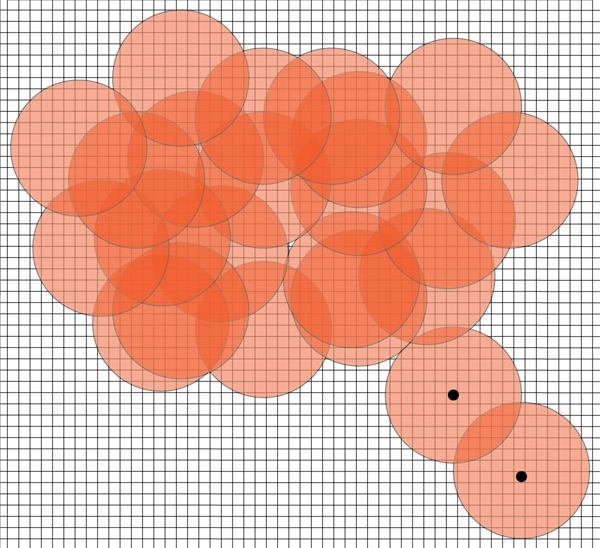
\includegraphics[width=10cm, height=10cm]{pic6}
    
       
        \end{figure}
    
    To overcome this issue, we apply a filtering on our dataset, within a specific zoom range where the overlaps occurs, in an attempt to reduce fake coloring of heatmaps.
    
    
    
    \subsection{ Markers on chuckholes Overlay}
    
    This feature was implemented to localize chuckholes that were detected during a bike ride. The locations are retrieved from the DataStore structure described previously. Using the Google Maps Android Marker Clustering Utility, a marker will be overlaid on the google map, on each location where the corresponding g-force level reaches or exceeds a specific threshold value = 3.5. 
    
    When a user views the map at a high zoom level, individual markers will be shown on the map. When a user zooms out, the markers gather together into clusters, to make viewing the map easier.
    \begin{figure}[H]
    \centering
	
	  
	   
       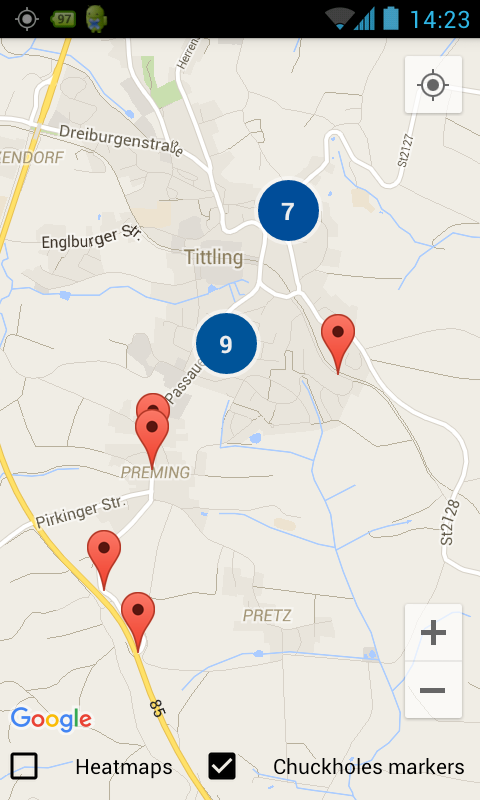
\includegraphics[width=5cm, height=8cm]{pic3}
    
       
        \end{figure}
    
    In case of no chuckhole in the area, the user will get a feedback via a toast message.
    

    
    

    
    
    
    
    
    
    
    
    
    
    
    
    
    
    % bib stuff
    \nocite{*}
    \addtocontents{toc}{\protect\vspace{\beforebibskip}}
    \addcontentsline{toc}{section}{\refname}    
    \bibliographystyle{plain}
    
    \bibliography{./Bibliography}
    %Google Maps Android API : %https://developers.google.com/maps/documentation/android-api
    
    %https://developer.android.com
    
    %Android Developers Blog : %http://android-developers.blogspot.de/
    
    %http://stackoverflow.com/
    
    
    
    
    
\end{document}
